%(BEGIN_QUESTION)
% Copyright 2009, Tony R. Kuphaldt, released under the Creative Commons Attribution License (v 1.0)
% This means you may do almost anything with this work of mine, so long as you give me proper credit

Examine this chromatogram showing several paraffinic hydrocarbon compounds (methane through pentane), and determine which peaks most likely belong to which compounds:

$$\includegraphics[width=15.5cm]{i04153x01.eps}$$

Use the label ``C1'' to refer to methane (CH$_{4}$), ``C2'' to refer to ethane (C$_{2}$H$_{6}$), ``C3'' to refer to propane (C$_{3}$H$_{8}$), etc.

\vskip 10pt

Identify which compounds experience the greatest {\it retention time}, and explain why they do.

\vskip 20pt \vbox{\hrule \hbox{\strut \vrule{} {\bf Suggestions for Socratic discussion} \vrule} \hrule}

\begin{itemize}
\item{} Identify a practical application for using a chromatograph to separate hydrocarbon compounds in a fluid stream.
\item{} Explain the significance of the ``flat-top'' peak shown in this chromatogram. 
\item{} Assuming this chromatogram was generated by a GC column at constant temperature, describe how it would change if {\it temperature programming} were included in the GC's configuration.
\end{itemize}

\underbar{file i04153}
%(END_QUESTION)





%(BEGIN_ANSWER)


%(END_ANSWER)





%(BEGIN_NOTES)

The lighter hydrocarbons (e.g. C1) come through the column first, while the heavier hydrocarbons (e.g. C5) come through last.

$$\includegraphics[width=15.5cm]{i04153x02.eps}$$

The larger the molecule, the greater the retention time, all other factors being equal.

%INDEX% Measurement, analytical: chromatography

%(END_NOTES)


